\documentclass[notitlepage]{revtex4-1}
\usepackage{geometry}
\usepackage{graphicx}
\usepackage{times}
\usepackage{physics}   % for simple physics notation
\usepackage{bm}        % for math
\usepackage{amssymb}   % for math
\usepackage{amsmath}
\usepackage{subfigure}
\usepackage{color}
\usepackage{float}
\usepackage{enumerate}
\usepackage{enumitem}
\usepackage[export]{adjustbox}
\usepackage{comment}
\usepackage{listings}
\usepackage{CJK}
\usepackage{graphicx}
\newcommand{\hilight}[1]{\colorbox{red}{#1}}
%\usepackage{physics}
%\usepackage{enumerate}
%\usepackage{booktabs} % not allowed in Revtex4.1
\begin{document}
\begin{CJK}{UTF8}{bsmi}
\title{First Principle 2017-Fall  Homework 1 Solution}
%\input author_list.tex       % D0 authors (remove the first 3 lines
                             % of this file prior to submission, they
                             % contain a time stamp for the authorlist)
                             % (includes institutions and visitors)
\author{Kai-Hsin Wu (吳愷訢)}
\email{r05222003@ntu.edu.tw}
\affiliation{Department of Physics and Center of Theoretical Sciences, National Taiwan University, Taipei 10607, Taiwan}

\date{\today}
\maketitle

\begin{enumerate}	
	\item The hcp structure is shown as following :
	
		\begin{figure}[!h]
			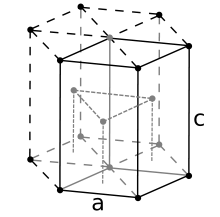
\includegraphics[width=4cm]{{Material/hcp}}
			\caption{hcp structure}
			\label{fig:hcp}
		\end{figure}
		we can calculate the c/a ratio as :
		\begin{equation*}
			\begin{split}
				x &\equiv \frac{c}{2} \\
				x &= \sqrt{ a^2 - (\frac{a}{\sqrt{3}})^2 } = a \cdot \sqrt{\frac{2}{3}} \\
				c/a &= 2 \sqrt{\frac{2}{3}}_{\#}
			\end{split}
		\end{equation*}	

	\item
		\begin{enumerate}[label=(\alph*)] 
			\item 
				\subitem for all $n_i \in$ even with primitive vectors $(2\hat{x} , 2\hat{y} , 2\hat{z})$ , the lattice is a simple cubic lattice with side length 2 origin at $(0\hat{x},0\hat{y},0\hat{z})$
				\subitem for all $n_i \in$ odd with primitive vectors $(2\hat{x} , 2\hat{y} , 2\hat{z})$ , the lattice is also a simple cubic lattice with side length 2 include point $(0\hat{x},0\hat{y},0\hat{z})$ 
			\item 
				\subitem In the case where $\sum_{i} n_i$ is even, this is a simple cubic lattice with side length $\sqrt{3}$ (which can be thought as a $\sqrt{3}$ scaled + $45^o$ rotated version of sc.)
		\end{enumerate}
	\item
		Let's defined the primitive reciprocal lattice is formed by $\langle G_1 , G_2 , G_3 \rangle$.  Which defined as :
		\begin{equation}
			\begin{split}
				G_i \cdot b_j = 2\pi \delta_{ij} 
			\end{split}
		\end{equation} 
		With the known relation:
		\begin{equation}
			\begin{split}
				b_i &\equiv \frac{2\pi (a_j \cross a_k)}{|a_1 \cdot (a_2 \cross a_3) |} \\
				a_i \cdot b_j &= 2\pi \delta_{ij}
			\end{split}
		\end{equation}
		we can see :
		\begin{equation}
			G_i = {a_i}_{\#} 
		\end{equation}			
			
	\item The honeycomb lattice is formed by primitive vectors as the same as parallelogram, with basis contain 2-sites. In which the reciprocal vectors also forms parallelogram. Since the Brillouin zone is just the Wigner-Seitz cell in reciprocal space. The Wigner-Seitz cell formed from parallelogram is hexagonal structure.    
	
	% 5
	\item 
	% 6
	\item 
		\begin{enumerate}[label=(\alph*)]
			\item $GaAs$ 
				\begin{figure}[!h]
					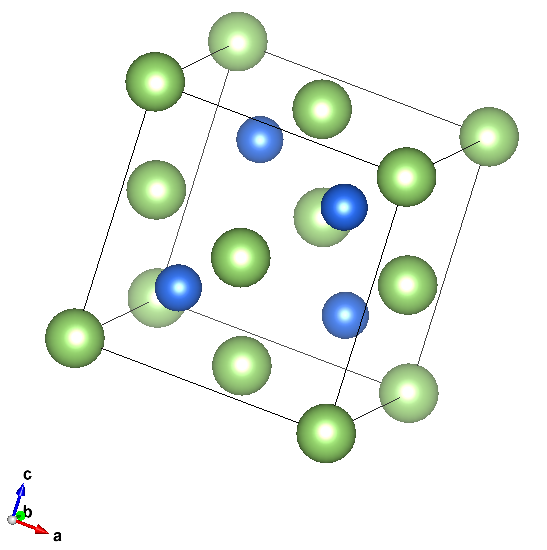
\includegraphics[width=4cm]{{Material/GaAs}}
					\caption{GaAs zinc-blende structure}
					\label{fig:gaas}
				\end{figure}
			
				POSCAR : 
				
\begin{lstlisting}
GaAs
5.653
1.000000000  0.000000000  0.000000000
0.000000000  1.000000000  0.000000000
0.000000000  0.000000000  1.000000000
Ga   As
4    4
Direct
0.000000000  0.000000000  0.000000000
0.000000000  0.500000000  0.500000000
0.500000000  0.500000000  0.000000000
0.500000000  0.000000000  0.500000000
0.750000000  0.250000000  0.750000000
0.250000000  0.250000000  0.250000000
0.250000000  0.750000000  0.750000000
0.750000000  0.750000000  0.250000000
\end{lstlisting}
			\newpage
			\item $NaCl$ 
				\begin{figure}[!h]
					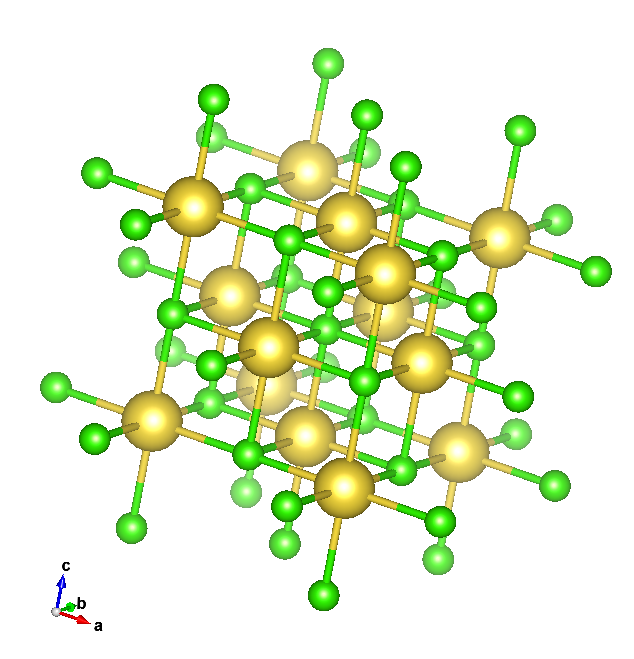
\includegraphics[width=4cm]{{Material/NaCl}}
					\caption{NaCl fcc structure}
					\label{fig:nacl}
				\end{figure}
				
				POSCAR :
\begin{lstlisting}
NaCl
5.64
1.000000000  0.000000000  0.000000000
0.000000000  1.000000000  0.000000000
0.000000000  0.000000000  1.000000000
Na  Cl
4   4
Direct
0.000000000  0.000000000  0.000000000
0.000000000  0.500000000  0.500000000
0.500000000  0.000000000  0.500000000
0.500000000  0.500000000  0.000000000
0.500000000  0.500000000  0.500000000
0.500000000  0.000000000  0.000000000
0.000000000  0.500000000  0.000000000
0.000000000  0.000000000  0.500000000
\end{lstlisting}	
			\newpage
			\item $SrTiO_3$
				\begin{figure}[!h]
					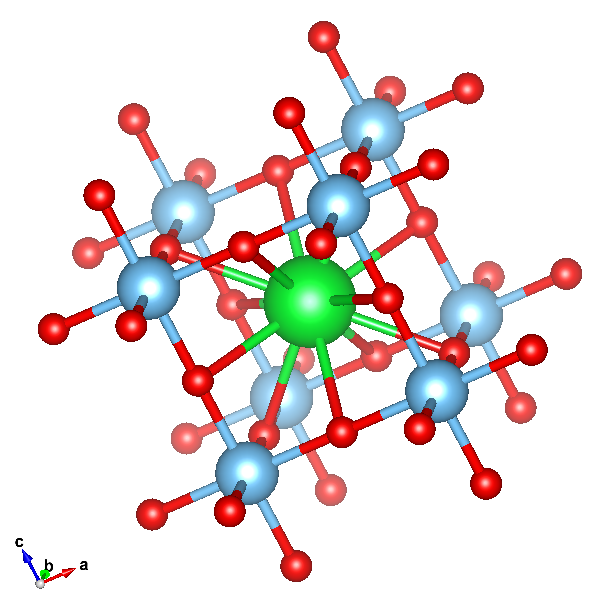
\includegraphics[width=4cm]{{Material/SrTiO3}}
					\caption{SrTiO3 sc structure}
					\label{fig:srtio3}
				\end{figure}
			
			POSCAR :
\begin{lstlisting}
SrTiO3
3.98805
1.000000000  0.000000000  0.000000000
0.000000000  1.000000000  0.000000000
0.000000000  0.000000000  1.000000000
Sr  Ti  O
1   1   3
Direct
0.500000000  0.500000000  0.500000000
0.000000000  0.000000000  0.000000000
0.500000000  0.000000000  0.000000000
0.000000000  0.500000000  0.000000000
0.000000000  0.000000000  0.500000000
\end{lstlisting}	
			\newpage
			\item $2H MoS_2$
				\begin{figure}[!h]
					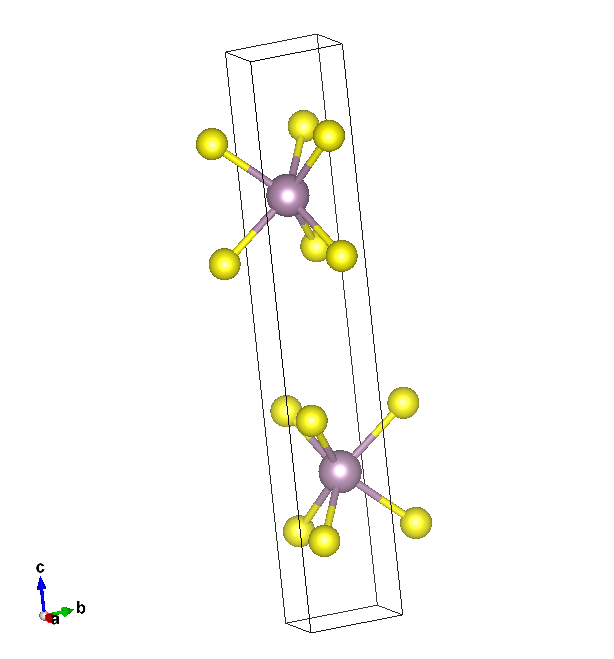
\includegraphics[width=4cm]{{Material/MoS2-2H}}
					\caption{MoS2-2H}
					\label{fig:mos22h}
				\end{figure}
			
			POSCAR :
\begin{lstlisting}
2H-MoS2
3.19
 1.000000000  0.000000000  0.000000000
-0.500000000  0.866025403  0.000000000
 0.000000000  0.000000000  4.664263323
Mo S
2 4
Direct
0.3333333333  0.666666667  0.250000000
0.6666666666  0.333333333  0.750000000
0.3333333333  0.666666667  0.855174000
0.3333333333  0.666666667  0.644826000
0.6666666666  0.333333333  0.355174000
0.6666666666  0.333333333  0.144826000
\end{lstlisting}			
		\end{enumerate}
	
	%7
	\item
	
	%8 
	\item Considering the block wave function $\psi_{n,\vec{k}}(r)$ with band index $n$, and wave vector$\vec{k}$. The Wannier functions center at lattice position $\vec{R}$ can be written in terms of inverse Fourier transform with constant $\kappa$ :
	\begin{equation}
		\begin{split}
			\phi_n(\vec{r} - \vec{R}) &= \kappa \sum_{\vec{k}} e^{-i \vec{k} \cdot \vec{R}} \psi_{n,\vec{k}}(\vec{r}) 
		\end{split}
	\end{equation}   
	
	Thus :
	\begin{equation}
		\begin{split}
			& \int \phi_n(\vec{r} - \vec{R})\phi_{n'}(\vec{r} - \vec{R}')  d^{D}\vec{r} \\
			&= \kappa^2 \sum_{\vec{k},\vec{h}} e^{i \vec{k} \cdot \vec{R}} e^{-i \vec{h} \cdot \vec{R}'} \int \psi^{*}_{n,\vec{k}}(\vec{r})\psi_{n',\vec{h}}(\vec{r}) d^{D}\vec{r} \\
			&= \kappa^2 \sum_{\vec{k},\vec{h}} e^{i \vec{k} \cdot \vec{R}} e^{-i \vec{h} \cdot \vec{R}'} \delta_{n,n'} \delta_{\vec{k},\vec{h}'} \\
			&= \kappa^2 \delta_{n,n'} \sum_{\vec{k}} e^{i \vec{k} \cdot (\vec{R}-\vec{R}')} \\
			&= \kappa^2 N \delta_{n,n'} \delta_{\vec{R},\vec{R}'} \\
			&\propto \delta_{n,n'} {\delta_{\vec{R},\vec{R}'}}_{\#}
		\end{split}
	\end{equation} 	
	
	The constant $\kappa$ can be derived by the normalization:
	
	\begin{align*}
	 &\int \phi_n(\vec{r} - \vec{R})\phi_{n'}(\vec{r} - \vec{R}') d^{D}\vec{r} = \delta_{n,n'} \delta_{\vec{R},\vec{R}'} \\
	 &\kappa^2 N = 1 \\
	 &\kappa = \frac{1}{\sqrt{N}}_{\#}
	\end{align*}

			
	
	
\end{enumerate}




\bibliographystyle{apsrev4-1}
\bibliography{ref}
	
\end{CJK}
\end{document}

